\documentclass{cls/resume}
\usepackage{sty/zh_CN-Adobefonts_external} 
\usepackage{sty/linespacing_fix}
\usepackage{cite}
\usepackage{graphicx}
\usepackage{textpos}
\usepackage{xcolor}
\usepackage{titlesec}

\begin{document}
\pagenumbering{gobble}

\name{某某某}
\contactInfo{\textit{手机}:(+86) 138-xxxx-xxxx}{\textit{性别}:男}{}{}
\contactInfo{\textit{邮箱}:example@email.com}{\textit{籍贯}:某省某市}{}{}

\begin{textblock*}{6cm}(-0.2cm, -2.9cm)
    
\includegraphics[width=6cm]{image/logo.png}
\end{textblock*}
\begin{textblock*}{2.5cm}(14.9cm, -2.9cm)
    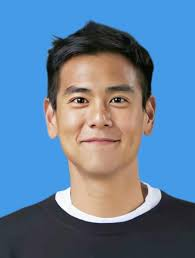
\includegraphics[width=2.5cm]{image/identification_photo.jpeg}
\end{textblock*}

\vspace{0.2cm} 

\section{教育背景}
\datedsubsection{\textbf{中国科学技术大学} | 计算机科学与技术 | \textit{硕士} | 985}{2023.9 - 2025.6}
\begin{itemize}[parsep=0.2ex]
    \item \textbf{荣誉}: 研究生国家奖学金\textbf{(Top 1\%)}
    \item \textbf{修习课程}: 深度学习理论与应用、高级机器学习、随机过程、最优化理论、分布式系统、计算理论
\end{itemize}
\datedsubsection{\textbf{中国科学技术大学} | 计算机科学与技术 | \textit{本科} | 985}{2019.9 - 2023.6}
\begin{itemize}[parsep=0.2ex]
    \item \textbf{GPA}: 4.25/4.3
    \item \textbf{荣誉}: \textbf{国家奖学金 (2次, Top 0.2\%)}、\textbf{安徽省优秀毕业生}、ACM-ICPC 国际大学生程序设计竞赛亚洲区域赛金奖、ACM-ICPC 国际大学生程序设计竞赛亚洲区域赛银奖、全国大学生数学建模竞赛国家一等奖、“挑战杯”全国大学生课外学术科技作品竞赛国家二等奖
    \item \textbf{修习课程}: 数据结构与算法、操作系统、计算机网络、编译原理、数据库系统、机器学习等
\end{itemize}

\section{论文发表}
\begin{itemize}
    \item Wang J, Li Y, Zhang M, et al. Rethinking Self-Attention: A Token-Mixing Approach for Vision Transformers[C]//International Conference on Learning Representations. Curran Associates, New York, 2024: 128-140.
\end{itemize}


\section{实习经历}
\datedsubsection{\textbf{某知名科技有限公司}, Research Internship}{2025.9-2025.12}
\begin{itemize}
    \item 独立负责车站地图开发(React),通过本地存储及JSBridge实现在全系应用中发布上线。
    \item 独立负责BU SPM chrome插件开发,支付成功/订单详情等页面的开发与交叉营销的接入工作。
\end{itemize}

\section{科研经历}
\datedsubsection{\textbf{基于检索增强生成的智能医疗问答系统}| \textbf{ICLR} 2025 | 一作}{2024.10-2025.5}
\begin{itemize}
  \item 针对大语言模型在专业领域(如医疗)中容易出现“幻觉”和知识更新不及时的问题,本项目设计并实现了一个基于 RAG 架构的智能问答系统。该系统旨在结合大模型的生成能力和外挂知识库的准确性,提供可靠的医疗信息咨询。
  \item 使用 Sentence-Transformer 对医疗知识库进行向量化处理,并存入 FAISS 向量数据库。当用户提问时,系统首先从数据库中检索最相关的文本片段,然后将其与原始问题一同输入给大语言模型(Llama),引导模型生成基于可靠知识的精准回答。实验证明,该方法准确率相比基线模型提升了15\%。
\end{itemize}

\datedsubsection{\textbf{基于改进YOLOv5的实时交通目标检测系统}}{2025.3-2025.7}
\begin{itemize}
  \item 为解决复杂交通场景下多尺度目标(尤其是小目标)检测精度低、速度慢的挑战,本项目对经典的 YOLOv5 算法进行了改进。通过引入注意力机制(CBAM)来增强网络对关键特征的关注度。
  \item 使用 BDD100K 数据集进行模型的训练与评估,并通过数据增强、迁移学习等策略提升模型的泛化能力。改进后的模型在保持实时检测速度(35 FPS)的同时,其平均精度均值(mAP)相较于基线 YOLOv5 提升了 4.5\%,尤其在车辆、行人等小目标的检测上效果显著。
\end{itemize}

\datedsubsection{\textbf{基于Seq2Seq与Attention机制的英汉机器翻译模型}}{2024.6-2024.8}
\begin{itemize}
  \item 为深入理解神经网络机器翻译的核心原理,本项目从零开始使用 PyTorch 搭建了一个包含编码器-解码器(Encoder-Decoder)的 Seq2Seq 翻译模型。编码器和解码器均采用 GRU 循环神经网络结构。
  \item 为解决长句子翻译过程中信息丢失的问题,在模型中引入了 Bahdanau 注意力机制,使解码器在生成每个目标词时能动态地关注源句的不同部分。在 WMT14 英汉翻译数据集上进行训练和测试,最终模型在测试集上达到了 23.6 的 BLEU 分数,验证了模型设计的有效性。
\end{itemize}

\section{技术能力}
\begin{itemize}[parsep=0.2ex]
    \item \textbf{技能}: Python, C, C++, Shell
    \item \textbf{语言}: 英语(IELTS, 7.5),德语(CET-6),普通话(母语)
    \item 熟悉 DeepSpeed框架多机多卡使用, vLLM推理加速框架, 模型量化等。
    \item \textbf{学生工作}: 院篮球队队长 (校冠军), 校学生会会长。
\end{itemize}

\end{document}
